%!TEX root = ../Main.tex

\chapter{Results}
An important aspect of HW/SW co-design is to identify potential bottlenecks of software tasks and to determine if that task is suitable for hardware acceleration. For this project it was determined that the calculation of distance between the points to be the most demanding task. On \cref{fig:algo_test_sw_pie} a pie chart shows the three most demanding tasks as the amount of clock cycles each process uses for one iteration of the genetic algorithm. It is seen that the 79\% of the clock cycles are spent on calculating the distances between points.

\Cref{fig:timing_pie_hw} shows the estimated distribution of clock cycles after HW-acceleration of the distance calculation. The estimate is found by multiplying the latency of the synthesized module which calculates the distance for one candidate solution with the population size. It is seen that after HW-acceleration, the calculation of distances accounts for only 8\% of the clock cycle utilization. The new "bottleneck" is the creation of generation, which could be HW-accelerated in a future iteration.

\Cref{fig:iterations_per_second} shows the iterations pr. second, comparing the full SW-implementation with the HW-accelerated implementation, with and without loop unrolling. In the full SW-implementation, the iterations pr second were approximated to around 1900. pr. second. For the HW-accelerated implementation with loop unrolling, this number is estimated to be around 6200. Thus, HW-acceleration of the distance-calculation results in an improvement of iterations pr. second of more than 200\%, which is a substantial increase.

The optimal loop unrolling factor for this implementation was found by means of trial and error, as described in \cref{sec:design_space_exploration}, and was found to be 3.

Even though the the group successfully synthesized and exported an IP core it was not possible to test the actual IP core on the ZYBO board. The reason for this was time constraints and would be an obvious thing to get working as future work.


\begin{figure}[H]
	\centering
	{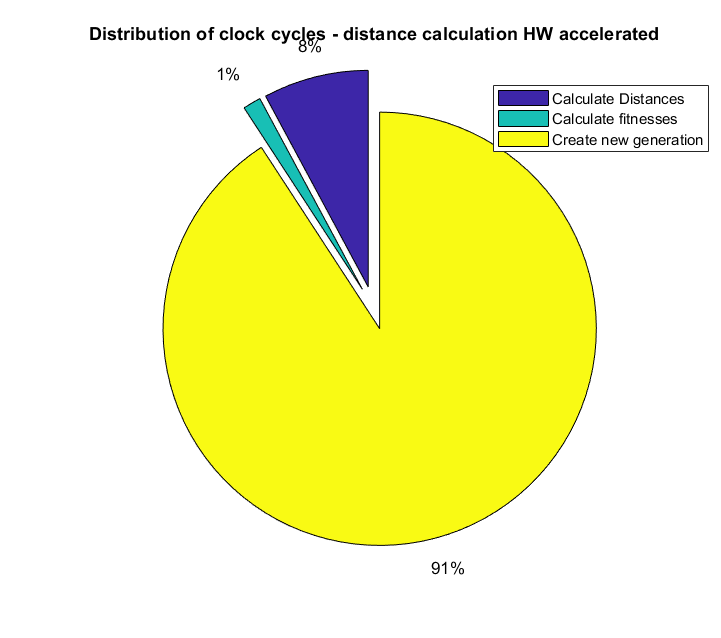
\includegraphics[width=\textwidth]{Images/cycle_distribution_HW_accelerated.png}}\\[0.5cm]
	\caption{Most demanding tasks in \% after hardware acceleration}
	\label{fig:timing_pie_hw}
\end{figure}

\Cref{fig:resource_utilization} shows the resources used by the module. It can be seen that it is well within the tolerated limits of the available resources, though it does use a substantial amount of resources.

\begin{figure}[H]
	\centering
	{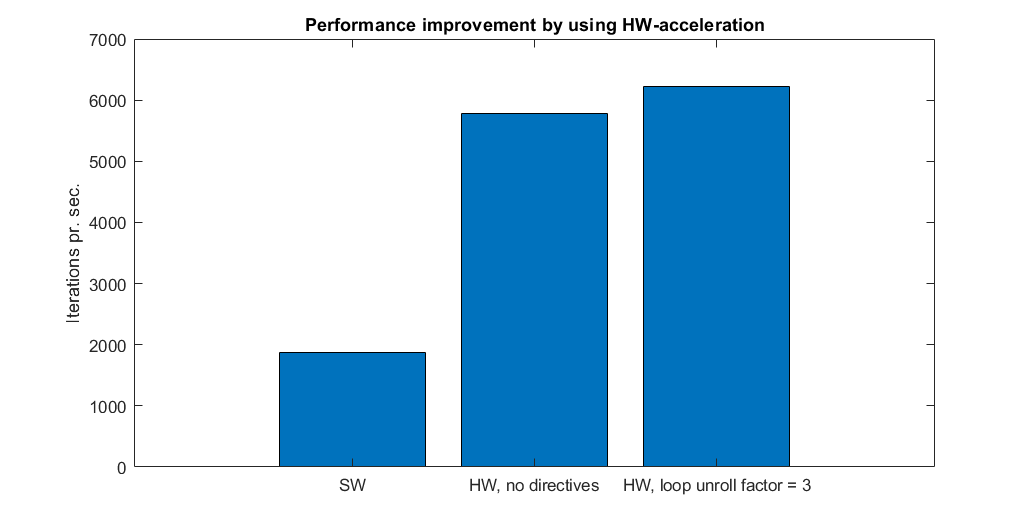
\includegraphics[width=\textwidth]{Images/performance_improvement_iterations_per_sec.png}}\\[0.5cm]
	\caption{Iterations pr. second, using different solutions.}
	\label{fig:iterations_per_second}
\end{figure}

\begin{figure}[H]
	\centering
	{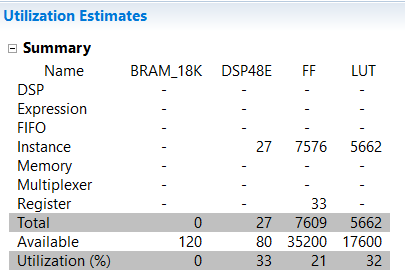
\includegraphics[width=\textwidth]{Images/resource_utilization_factor3.png}}\\[0.5cm]
	\caption{Resource utilization when using unroll factor=3.}
	\label{fig:resource_utilization}
\end{figure}